\documentclass[letterpaper,11pt]{article}

% Basado en la plantilla académica proporcionada por Josué Martínez.
\usepackage{silence}
\WarningFilter{babel}{Command \showhyphens}
\usepackage[T1]{fontenc}
\usepackage[utf8]{inputenc}
\usepackage[spanish,es-nodecimaldot]{babel}
\usepackage{amsmath,amssymb,mathtools}
\usepackage{graphicx}
\usepackage{csquotes}
\usepackage{geometry}
\usepackage{fancyhdr}
\usepackage[hidelinks]{hyperref}
\usepackage{parskip}
\usepackage{array}
\usepackage{booktabs}
\usepackage{enumitem}
\usepackage{microtype}
\usepackage{caption}
\usepackage{float}
\usepackage[backend=biber,style=numeric,sorting=none]{biblatex}
\addbibresource{referencias.bib}

% ============================================================
% DATOS DE LA INVESTIGACIÓN
% ============================================================
\newcommand{\universidad}{Universidad de San Carlos de Guatemala}
\newcommand{\escuela}{Escuela de Ciencias Físicas y Matemáticas}
\newcommand{\estudiante}{Josué Martínez}
\newcommand{\carne}{202104946}
\newcommand{\curso}{Relatividad General}
\newcommand{\profesor}{Dr. Juan Ponciano}
\newcommand{\numerotarea}{Informe de investigación}
\newcommand{\titulotarea}{Soluciones de Friedmann para universos con curvatura espacial}
\newcommand{\fechatarea}{16 de noviembre de 2026}
\newcommand{\logousac}{logo_usac.png}
\newcommand{\logoecfm}{logo_ecfm.png}

\geometry{top=4.0cm,bottom=2.0cm,left=2.0cm,right=2.0cm,headheight=2.9cm,headsep=0.3cm}
\setlength{\parskip}{3pt}
\setlength{\parindent}{0pt}
\setlength{\abovedisplayskip}{5pt}
\setlength{\belowdisplayskip}{5pt}
\setlength{\abovedisplayshortskip}{3pt}
\setlength{\belowdisplayshortskip}{3pt}
\setlist[itemize]{topsep=3pt,itemsep=2pt}
\setlist[enumerate]{topsep=3pt,itemsep=2pt}
\AtBeginBibliography{\footnotesize}
\setlength{\bibitemsep}{1pt}
\captionsetup{font=small,labelfont=bf}
\graphicspath{{figuras/}}

\fancypagestyle{tarea}{%
  \fancyhf{}
  \fancyhead[L]{\includegraphics[width=2.1cm]{\logousac}}
  \fancyhead[C]{%
    \begin{minipage}[b]{0.60\textwidth}
      \raggedright
      \universidad\\
      \escuela\\
      \estudiante{} -- Carné: \carne\\
      \curso\\
      \profesor
    \end{minipage}}
  \fancyhead[R]{\includegraphics[width=1.8cm]{\logoecfm}}
  \fancyfoot[C]{\thepage}
  \renewcommand{\headrulewidth}{0pt}
}
\fancypagestyle{continuacion}{%
  \fancyhf{}
  \fancyhead[L]{\small\bfseries \numerotarea}
  \fancyhead[R]{\small\bfseries \curso}
  \fancyfoot[C]{\thepage}
  \renewcommand{\headrulewidth}{0pt}
}
\newcommand{\encabezadotarea}{%
  \pagestyle{continuacion}
  \thispagestyle{tarea}
  \hrule height 1.3pt
  \vspace{0.18cm}
  \begin{center}
    {\Large\bfseries \titulotarea}\\[0.05cm]
    {\small Estudio analítico y comprobación numérica de modelos FLRW}\\[0.05cm]
    {\small \fechatarea}
  \end{center}
  \vspace{0.18cm}
  \hrule height 1.3pt
  \vspace{0.22cm}
}
\newcommand{\td}{\mathrm{d}}
\newcommand{\Rthree}{\prescript{(3)}{}{R}}
\newcommand{\dd}{\mathop{}\!\mathrm{d}}

\begin{document}
\encabezadotarea

\begin{abstract}
\noindent
Se estudian soluciones de las ecuaciones de Friedmann para universos homogéneos e isótropos con curvatura espacial positiva, nula y negativa. Para aislar el papel del parámetro de curvatura se adopta un fluido de materia sin presión y constante cosmológica nula. Se obtienen la solución de potencia del modelo plano y las soluciones paramétricas de los modelos cerrado y abierto; posteriormente se integran las ecuaciones adimensionales mediante el método DOP853 de SciPy. La comparación entre soluciones exactas y numéricas arroja errores absolutos máximos entre $10^{-9}$ y $10^{-12}$, mientras que la restricción de Friedmann permanece satisfecha con residuos pequeños. Se discuten los resultados físicos, las verificaciones realizadas y las limitaciones de estos modelos idealizados.
\end{abstract}
\textbf{Palabras clave:} cosmología FLRW, curvatura espacial, ecuaciones de Friedmann, integración numérica, DOP853.

\par\smallskip
\noindent\textbf{Repositorio del proyecto:}
\href{https://github.com/Exoid523/friedmann-curvatura-espacial}
{\texttt{github.com/Exoid523/friedmann-curvatura-espacial}}

\section{Introducción y objetivos}

Las ecuaciones de Einstein permiten relacionar la geometría del espacio-tiempo con su contenido de materia y energía. Bajo las hipótesis de homogeneidad e isotropía espaciales, la geometría adopta la forma de Friedmann--Lemaître--Robertson--Walker (FLRW), cuyo comportamiento dinámico se describe mediante un factor de escala $a(t)$. La cosmología relativista resulta así un ejemplo accesible de aplicación de las ecuaciones de campo de Einstein a un sistema con simetrías relevantes \cite{janssen2013,carroll2004,weinberg1972}.

El propósito de esta investigación es comparar tres geometrías espaciales normalizadas, $k=+1,0,-1$, bajo un mismo modelo de materia. Se persiguen tres objetivos concretos: derivar las soluciones analíticas correspondientes, construir una integración numérica independiente de las trayectorias e interpretar la influencia de la curvatura espacial a partir de las soluciones y de las verificaciones matemáticas.

El alcance se restringe a universos dominados por materia no relativista sin presión ($p=0$), con densidad positiva y constante cosmológica nula ($\Lambda=0$). Esta elección permite obtener expresiones exactas y contrastarlas directamente con un algoritmo numérico. No se pretende ajustar parámetros observacionales ni describir la composición completa del universo actual.

\section{Formulación geométrica y ecuaciones de Friedmann}

Adoptamos la signatura métrica $(+,-,-,-)$ utilizada en el curso. La métrica FLRW, con $r$ adimensional y $a(t)$ expresado en unidades de longitud, es
\begin{equation}
\boxed{\dd s^2=c^2\dd t^2-a^2(t)\left[\frac{\dd r^2}{1-kr^2}+r^2(\dd\theta^2+\sin^2\theta\,\dd\phi^2)\right].}
\label{eq:flrw}
\end{equation}
El parámetro $k$ representa la curvatura espacial normalizada y la curvatura escalar intrínseca de las secciones $t=\mathrm{cte}$ es
\begin{equation}
\Rthree=\frac{6k}{a^2(t)}.
\label{eq:3curv}
\end{equation}
Por ello, $k=+1$ corresponde a curvatura positiva, $k=0$ a secciones planas y $k=-1$ a curvatura negativa. Estos nombres se refieren a la \emph{geometría espacial}, no directamente a la topología global ni, sin hipótesis adicionales, al destino dinámico del universo.

Para la materia utilizamos un fluido perfecto con tensor energía-momento $T^\mu{}_\nu=\operatorname{diag}(\rho c^2,-p,-p,-p)$ en las coordenadas comóviles. La inserción de \eqref{eq:flrw} en las ecuaciones de Einstein conduce a
\begin{align}
H^2&=\frac{8\pi G}{3}\rho-\frac{kc^2}{a^2}+\frac{\Lambda c^2}{3}, \label{eq:friedmann1}\\
\frac{\ddot a}{a}&=-\frac{4\pi G}{3}\left(\rho+\frac{3p}{c^2}\right)+\frac{\Lambda c^2}{3},\label{eq:friedmann2}
\end{align}
donde $H=\dot a/a$ es el parámetro de Hubble y $\rho$ la densidad de masa. La conservación covariante, $\nabla_\mu T^{\mu\nu}=0$, proporciona la ecuación de continuidad
\begin{equation}
\dot\rho+3\frac{\dot a}{a}\left(\rho+\frac{p}{c^2}\right)=0.
\label{eq:continuidad}
\end{equation}
Las tres ecuaciones contienen información relacionada: con las hipótesis del fluido y la conservación, las ecuaciones de expansión y aceleración no son independientes \cite{janssen2013,carroll2004}.

\subsection{Reducción al modelo de materia}

Para $p=0$, la ecuación \eqref{eq:continuidad} se integra mediante separación de variables,
\[
\frac{\dd\rho}{\rho}=-3\frac{\dd a}{a}
\quad\Longrightarrow\quad
\rho a^3=\rho_0a_0^3.
\]
El subíndice $0$ indica un instante de referencia arbitrario. Si, además, $\Lambda=0$, entonces \eqref{eq:friedmann1} da
\begin{align*}
\frac{\dot a^2}{a^2}
&=\frac{8\pi G}{3}\frac{\rho_0a_0^3}{a^3}-\frac{kc^2}{a^2},\\
\dot a^2&=\frac{C}{a}-kc^2,
\qquad C\equiv\frac{8\pi G}{3}\rho_0a_0^3>0.
\end{align*}
Así obtenemos la ecuación central del estudio:
\begin{equation}
\boxed{\dot a^2=\frac{C}{a}-kc^2.}
\label{eq:central}
\end{equation}
El análisis dimensional verifica que $[C]=\mathrm{m^3\,s^{-2}}$, de modo que ambos lados de \eqref{eq:central} tienen unidades de $\mathrm{m^2\,s^{-2}}$. Su derivada temporal, donde $\dot a\neq0$, implica
\[
2\dot a\ddot a=-\frac{C}{a^2}\dot a
\quad\Longrightarrow\quad
\boxed{\ddot a=-\frac{C}{2a^2}<0.}
\]
La relación se mantiene por continuidad en el punto de máxima expansión del modelo cerrado. En consecuencia, los tres modelos presentan aceleración negativa, aunque sus velocidades de expansión no sean iguales.

\subsection{Variables adimensionales}

Para utilizar las mismas escalas en los tres casos definimos
\begin{equation}
a_* =\frac{C}{2c^2},\qquad
 t_* =\frac{C}{2c^3},\qquad
 x=\frac{a}{a_*},\qquad \tau=\frac{t}{t_*}.
\label{eq:escalas}
\end{equation}
Como $a_*/t_*=c$, se cumple $\dot a=c\,\td x/\td\tau$. Además, $C/a=2c^2/x$. Por tanto, \eqref{eq:central} y su ecuación de aceleración se escriben como
\begin{equation}
\boxed{\left(\frac{\td x}{\td\tau}\right)^2=\frac{2}{x}-k,\qquad
\frac{\td^2x}{\td\tau^2}=-\frac{1}{x^2}.}
\label{eq:adimensionales}
\end{equation}
La primera expresión constituye una restricción que deben satisfacer las condiciones iniciales; la segunda describe la evolución una vez fijadas dichas condiciones.

\section{Soluciones analíticas}

\subsection{Curvatura nula: $k=0$}

La ecuación \eqref{eq:central} en la rama expansiva toma la forma $\td a/\td t=\sqrt{C/a}$. Separando e integrando,
\[
a^{1/2}\dd a=\sqrt C\dd t,
\qquad \frac{2}{3}a^{3/2}=\sqrt C\,(t-t_B),
\]
donde $t_B$ es la constante de integración que fija el origen de la expansión. Tomando $t_B=0$ y despejando,
\begin{equation}
\boxed{a(t)=\left(\frac{9C}{4}\right)^{1/3}t^{2/3},\qquad
x(\tau)=\left(\frac{9}{2}\tau^2\right)^{1/3}.}
\label{eq:plano}
\end{equation}
Esto implica $H=2/(3t)$ y $\ddot a=-2a/(9t^2)<0$: la expansión continúa para $t>0$, pero se desacelera. La sustitución de \eqref{eq:plano} en \eqref{eq:central} reproduce exactamente $\dot a^2=C/a$.

\subsection{Curvatura positiva: $k=+1$}

En este caso $\dot a^2=C/a-c^2$. La condición $\dot a^2\geq0$ impone $0<a\leq C/c^2$. Para integrar introducimos el tiempo conforme adimensional $\eta$ mediante
\[
\dd\eta=\frac{c\,\dd t}{a},\qquad
\left(\frac{\td a}{\td\eta}\right)^2=\frac{C}{c^2}a-a^2.
\]
Definiendo $A=C/c^2$, elegimos la sustitución $a=A\sin^2(\eta/2)$, ya que
\[
\left(\frac{\td a}{\td\eta}\right)^2
=\frac{A^2}{4}\sin^2\eta
=a(A-a).
\]
La relación entre $t$ y $\eta$ se obtiene de $\td t=(a/c)\td\eta$:
\begin{equation}
\boxed{a(\eta)=\frac{A}{2}(1-\cos\eta),\qquad
 t(\eta)=\frac{A}{2c}(\eta-\sin\eta).}
\label{eq:cerradofis}
\end{equation}
En las variables de \eqref{eq:escalas},
\begin{equation}
\boxed{x(\eta)=1-\cos\eta,\qquad \tau(\eta)=\eta-\sin\eta,\quad 0\leq\eta\leq2\pi.}
\label{eq:cerrado}
\end{equation}
La derivada temporal es $\dot a=c\cot(\eta/2)$; por ello, el máximo se alcanza en $\eta=\pi$. La solución predice
\begin{equation}
a_{\max}=\frac{C}{c^2},\qquad
x_{\max}=2,\qquad
\tau_{\max}=\pi,\qquad
\tau_{\rm final}=2\pi.
\label{eq:maximo}
\end{equation}
La solución parte de $a=0$, se expande hasta el máximo y luego se contrae. Este recolapso es consecuencia de las hipótesis $p=0$, $\Lambda=0$ y $k=+1$; no debe atribuirse de manera universal a toda geometría espacial cerrada.

\subsection{Curvatura negativa: $k=-1$}

La ecuación para $a(\eta)$ ahora es
\[
\left(\frac{\td a}{\td\eta}\right)^2=Aa+a^2.
\]
La sustitución hiperbólica $a=A\sinh^2(\eta/2)$ satisface la ecuación porque
\[
\left(\frac{\td a}{\td\eta}\right)^2=\frac{A^2}{4}\sinh^2\eta=a(A+a).
\]
Integrando la relación temporal $\td t=(a/c)\td\eta$ obtenemos
\begin{equation}
\boxed{a(\eta)=\frac{A}{2}(\cosh\eta-1),\qquad
 t(\eta)=\frac{A}{2c}(\sinh\eta-\eta).}
\label{eq:abiertofis}
\end{equation}
En variables adimensionales,
\begin{equation}
\boxed{x(\eta)=\cosh\eta-1,\qquad \tau(\eta)=\sinh\eta-\eta,\quad\eta\geq0.}
\label{eq:abierto}
\end{equation}
La velocidad $\dot a=c\coth(\eta/2)>0$ no se anula. Para $\eta\gg1$, las funciones hiperbólicas crecen proporcionalmente a $e^\eta$, por lo que $a(t)\sim ct$, o $x(\tau)\sim\tau$: la expansión se aproxima a una ley lineal a tiempos grandes.

\subsection{Comportamiento inicial común}

Las expansiones de Taylor $1-\cos\eta\simeq\eta^2/2$, $\cosh\eta-1\simeq\eta^2/2$, $\eta-\sin\eta\simeq\eta^3/6$ y $\sinh\eta-\eta\simeq\eta^3/6$ muestran que las soluciones con $k=\pm1$ satisfacen
\[
x\simeq\frac{\eta^2}{2},\qquad \tau\simeq\frac{\eta^3}{6}.
\]
Eliminando $\eta$ se recupera $x\sim(9\tau^2/2)^{1/3}$, igual que en el caso plano. En este régimen, el término de materia $2/x$ domina frente al término de curvatura $k$.

\section{Implementación y verificaciones numéricas}

\subsection{Sistema diferencial y condiciones iniciales}

Definimos $v=\td x/\td\tau$ y utilizamos el sistema de primer orden
\begin{equation}
\boxed{\frac{\td}{\td\tau}\begin{pmatrix}x\\v\end{pmatrix}
=\begin{pmatrix}v\\-x^{-2}\end{pmatrix}.}
\label{eq:sistema}
\end{equation}
La curvatura $k$ no aparece de manera explícita en el segundo miembro: determina las condiciones iniciales admisibles mediante la restricción $v_0^2=2/x_0-k$. Para comparar los modelos se tomó $x_0=0.5$ y la rama inicialmente expansiva,
\begin{equation}
v_0=\sqrt{4-k}=\begin{cases}
\sqrt3,&k=+1,\\
2,&k=0,\\
\sqrt5,&k=-1.
\end{cases}
\label{eq:condiciones}
\end{equation}
El origen $\tau=0$ de la integración corresponde por tanto a $x=0.5$, no a la singularidad inicial del modelo analítico.

La ecuación \eqref{eq:sistema} se integró con \texttt{scipy.integrate.solve\_ivp}, utilizando \texttt{DOP853}, un esquema explícito de Runge--Kutta de orden ocho con control adaptativo del error \cite{scipyivp,virtanen2020}. Se utilizaron los parámetros de la tabla \ref{tab:parametros}.

\begin{table}[htbp]
\centering\small
\caption{Configuración del cálculo numérico reproducido.}
\label{tab:parametros}
\begin{tabular}{@{}ll@{}}
\toprule
Parámetro & Valor \\
\midrule
Método & DOP853 \\
Tolerancia relativa y absoluta & $10^{-10}$ y $10^{-12}$ \\
Paso máximo permitido & $0.02$ (tiempo adimensional) \\
Intervalo de integración & $0\leq\tau\leq6.5$ \\
Condición inicial & $x_0=0.5$, $v_0=\sqrt{4-k}$ \\
Evento para la rama contractiva & detener cuando $x$ desciende a $0.05$ \\
\bottomrule
\end{tabular}
\end{table}

La integración numérica se detiene antes de la singularidad $x=0$. Para el modelo cerrado el evento se activó en $\tau\simeq6.096703$ medido desde $x_0=0.5$, mientras que los modelos plano y abierto alcanzaron $\tau=6.5$. El punto de máxima expansión del modelo cerrado puede atravesarse sin cambiar de ecuación diferencial, ya que el sistema \eqref{eq:sistema} es regular allí.

\subsection{Comparación con las soluciones exactas}

Para comparar cada trayectoria se evaluó la solución analítica en los mismos instantes de la solución numérica. Fue necesario trasladar el origen temporal de las expresiones analíticas. En el caso plano,
\begin{equation}
\tau_{0,\mathrm{plano}}=\sqrt{\frac{2x_0^3}{9}},\qquad
x_{\rm exacto}(\tau)=\left[\frac92(\tau+\tau_{0,\mathrm{plano}})^2\right]^{1/3}.
\end{equation}
Para el modelo cerrado se calculó $\eta_0=\arccos(1-x_0)$, y para el abierto $\eta_0=\operatorname{arcosh}(1+x_0)$. Las relaciones $\tau(\eta)$ se desplazaron mediante el valor correspondiente de $\tau(\eta_0)$ antes de evaluar $x_{\rm exacto}$. En esos dos casos, la evaluación analítica sobre los tiempos del integrador se efectuó mediante interpolación lineal de un muestreo paramétrico de $50\,000$ puntos.

Se definió el error absoluto máximo
\begin{equation}
E_{\max}=\max_i\left|x_{\rm num}(\tau_i)-x_{\rm exacto}(\tau_i)\right|.
\label{eq:error}
\end{equation}
Como segunda prueba se calculó el residuo de la restricción de Friedmann en cada punto de la trayectoria,
\begin{equation}
\epsilon_i=v_i^2-\frac{2}{x_i}+k,\qquad
\epsilon_{\max}=\max_i|\epsilon_i|.
\label{eq:residuo}
\end{equation}
Ambas verificaciones son complementarias: la primera compara con una referencia analítica, mientras que la segunda comprueba el cumplimiento de una primera integral del sistema.

\section{Resultados}

\subsection{Evolución del factor de escala}

La figura \ref{fig:analiticas} presenta las tres soluciones analíticas, usando las mismas variables y escalas adimensionales. El caso cerrado alcanza $x=2$ en $\tau=\pi$ y vuelve a $x=0$ en $\tau=2\pi$. Los modelos plano y abierto continúan expandiéndose; para igual $\tau>0$, el modelo abierto alcanza valores mayores del factor de escala en la normalización adoptada. Las curvas comienzan con un comportamiento semejante y se separan conforme avanza la evolución.

\begin{figure}[htbp]
\centering
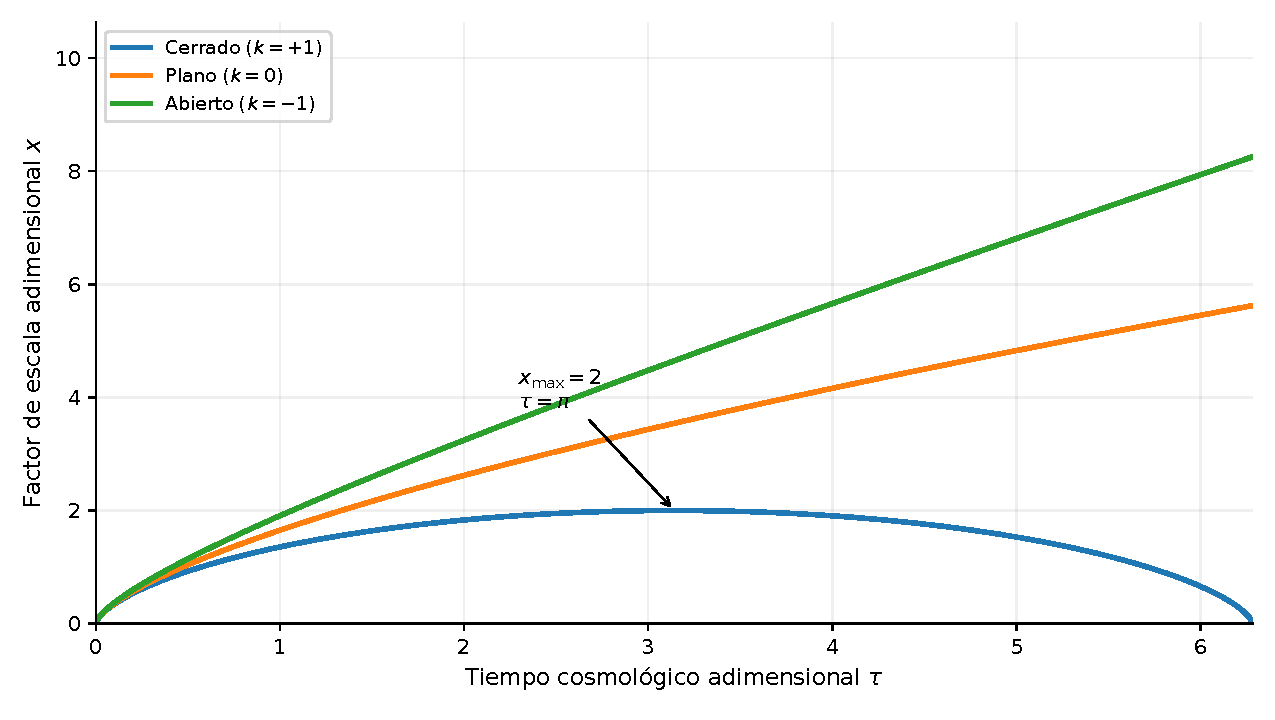
\includegraphics[width=0.94\textwidth]{friedmann_analiticas.pdf}
\caption{Evolución analítica del factor de escala adimensional para $k=+1,0,-1$, a partir de las ecuaciones \eqref{eq:plano}, \eqref{eq:cerrado} y \eqref{eq:abierto}. El punto señalado es el máximo del modelo cerrado.}
\label{fig:analiticas}
\end{figure}

\subsection{Concordancia analítica--numérica}

La figura \ref{fig:comparacion} muestra las soluciones exactas junto con los resultados obtenidos mediante DOP853. El eje horizontal representa el tiempo transcurrido desde la condición inicial $x_0=0.5$ y no desde el origen de cada solución paramétrica. Los puntos numéricos se superponen con las curvas exactas, incluido el máximo de expansión y la fase contractiva del modelo cerrado.

\begin{figure}[htbp]
\centering
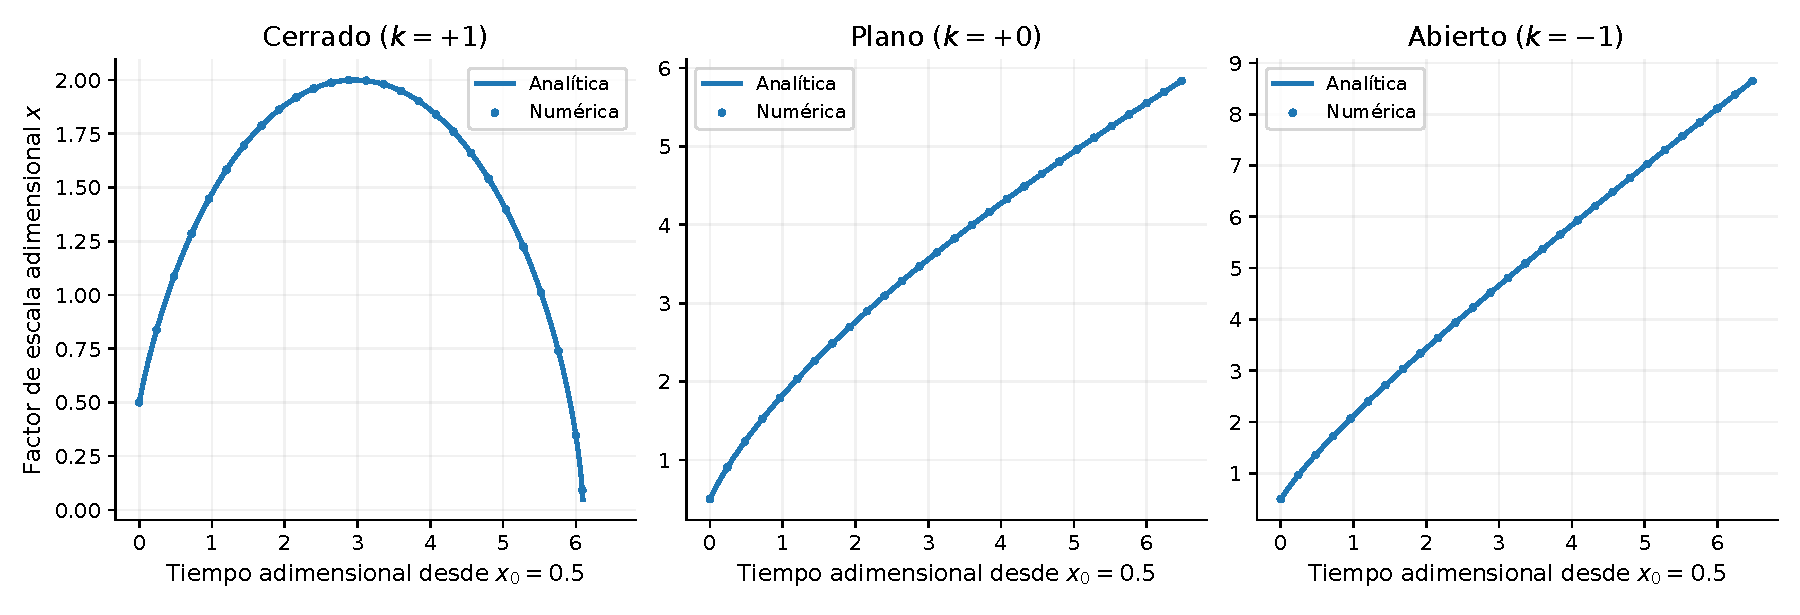
\includegraphics[width=\textwidth]{friedmann_comparacion.pdf}
\caption{Comparación de soluciones analíticas (línea) y numéricas (puntos) para cada valor de $k$. Se aplicó el corrimiento de origen temporal correspondiente a $x_0=0.5$. El modelo cerrado se detuvo antes del colapso singular, en $x=0.05$.}
\label{fig:comparacion}
\end{figure}

Los errores registrados en el archivo \texttt{resultados/errores\_friedmann.csv}, generado por el programa, se resumen en la tabla \ref{tab:errores}. Los valores se presentan con un número moderado de cifras significativas porque el objetivo es caracterizar el orden de magnitud de la discrepancia.

\begin{table}[htbp]
\centering
\caption{Errores absolutos máximos y residuos de la restricción, obtenidos en las ejecuciones del proyecto.}
\label{tab:errores}
\begin{tabular}{@{}lcc@{}}
\toprule
Modelo & $E_{\max}$ & $\epsilon_{\max}$ \\
\midrule
Cerrado, $k=+1$ & $1.370463\times10^{-9}$ & $2.106056\times10^{-9}$ \\
Plano, $k=0$ & $4.093614\times10^{-12}$ & $1.198375\times10^{-12}$ \\
Abierto, $k=-1$ & $4.610599\times10^{-10}$ & $2.211009\times10^{-12}$ \\
\bottomrule
\end{tabular}
\end{table}

La concordancia es buena en los tres casos para el intervalo integrado. El error reportado en $E_{\max}$ no es una medida aislada del error del integrador: los modelos con $k=\pm1$ incluyen el error de la interpolación paramétrica utilizada para evaluar la solución exacta. Por otra parte, los residuos $\epsilon_{\max}$ indican que la restricción inicial se mantiene aproximadamente durante la evolución numérica. No se ha realizado un estudio sistemático de convergencia al variar las tolerancias y el paso máximo, por lo que no se atribuye a estos resultados una garantía de exactitud fuera del experimento realizado.

\section{Discusión física y limitaciones}

El análisis permite separar dos ideas que podrían confundirse. La ecuación de aceleración $x''=-x^{-2}$ es idéntica para los tres modelos y expresa la desaceleración producida por la materia. La diferencia cualitativa entre las trayectorias proviene de la restricción $v^2=2/x-k$: para $k=+1$ existe un punto donde $v=0$, mientras que para $k=0$ y $k=-1$ la rama en expansión no tiene un máximo del factor de escala dentro del modelo considerado.

La distinción entre geometría espacial y evolución dinámica es esencial. La clasificación abierto, plano y cerrado se refiere al signo de $\Rthree$ y, por sí sola, no determina el comportamiento de una solución cosmológica general. Aquí el recolapso del modelo cerrado es consecuencia conjunta del valor $k=+1$ y de la elección $p=0$, $\Lambda=0$. Con una constante cosmológica o componentes adicionales, las conclusiones pueden cambiar.

El cálculo numérico también tiene restricciones concretas. Se integra una ecuación homogénea e isótropa sin perturbaciones, con parámetros adimensionales fijados para facilitar la comparación y sin observaciones astronómicas. Además, el integrador evita el punto singular $x=0$ y la comparación de modelos con curvatura recurre a una interpolación finita. Estas decisiones son apropiadas para verificar las soluciones analíticas, pero limitan la interpretación de los errores y excluyen, por ejemplo, un estudio detallado de la singularidad cosmológica.

\section{Conclusiones}

La reducción de las ecuaciones de Einstein al modelo FLRW con materia sin presión permitió expresar los tres casos de curvatura mediante una sola ecuación diferencial. El modelo plano produjo la ley $a\propto t^{2/3}$; el cerrado presentó una solución trigonométrica con expansión máxima y recolapso; y el abierto condujo a una solución hiperbólica con expansión indefinida.

La integración independiente del sistema adimensional mediante DOP853 reprodujo estas trayectorias. Los errores máximos respecto de las referencias analíticas se situaron aproximadamente entre $10^{-9}$ y $10^{-12}$ y los residuos de la restricción de Friedmann se mantuvieron pequeños para los parámetros utilizados.

La comparación muestra que, aun con la misma ecuación de aceleración, el signo de la curvatura modifica las velocidades admisibles y la evolución global en el modelo estudiado. La consistencia de las soluciones se comprobó mediante dos procedimientos complementarios, sin recurrir a un ajuste de parámetros observacionales.

\section*{Reproducibilidad del cálculo}

La implementación se organizó en tres archivos principales: \texttt{src/soluciones\_analiticas.py} contiene las expresiones exactas; \texttt{src/soluciones\_numericas.py} resuelve el sistema con \texttt{solve\_ivp}; y \texttt{main.py} genera las gráficas y exporta el archivo \texttt{resultados/errores\_friedmann.csv}. Las figuras se guardan en formatos PNG y PDF. El repositorio local incluye además un \texttt{README.md} con los parámetros del modelo, dependencias e instrucciones de ejecución. La reproducción gráfica de este informe utiliza los mismos parámetros e incorpora el código correspondiente entre los archivos fuente adjuntos.

% Bibliografía al final en hoja independiente (convención de la plantilla).
\clearpage
\printbibliography[title={Referencias}]
\end{document}
